\section{Рекурсивные вычисления}
\textbf{Задание:} Создать рекурсивную функцию, которая для заданного целого $n$
вычисляет сумму ряда $\displaystyle \sum\limits_{i=1}^n 2^i$

Для этого были использовано 3 элемента Label, 2 элемента TextBox, 1 элемент PictureBox
и один элемент Button. 

Создано окно, содержащее три элемента TextBox, три элемента Label и 
один элемент Button. После запуска приложения появляется окно (см. рисунок \ref{fig:form3}) .
\begin{figure}[H]
    \centering
    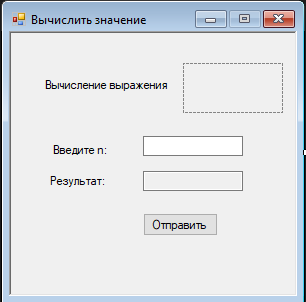
\includegraphics{task3/form.png}
    \caption{Внешний вид формы в конструкторе}
    \label{fig:form3}
\end{figure}

У элементов изменены значения некоторых атрибутов. 
Значения измененных атрибутов представлены в таблице \ref{table:params3}.

\begin{table}[H]
    \small
    \caption{Значения атрибутов элементов в приложении <<Рекурсивные вычисления>>}
    \begin{tabular}{|l|l|}\hline
    Наименование атрибута & Значение\cr\hline
    \multicolumn{2}{|l|}{Для формы}\cr\hline
    \verb"Text" & \verb"Вычислить значение"\cr\hline
    \verb"FormBorderStyle" & \verb"FixedSingle"\cr\hline
    \verb"MaximizeBox" & \verb"False"\cr\hline
    \multicolumn{2}{|l|}{Для первой надписи}\cr\hline
    \verb"(Name)" & \verb"formulaText"\cr\hline
    \verb"Text" & \verb"Вычисление выражения"\cr\hline
    \multicolumn{2}{|l|}{Для второй надписи}\cr\hline
    \verb"(Name)" & \verb"xLabel"\cr\hline
    \verb"Text" & \verb"Введите N"\cr\hline
    \multicolumn{2}{|l|}{Для третьей надписи}\cr\hline
    \verb"(Name)" & \verb"lblOutput"\cr\hline
    \verb"Text" & \verb"Результат:"\cr\hline
    \multicolumn{2}{|l|}{Для первого текстового поля}\cr\hline
    \verb"(Name)" & \verb"xInput"\cr\hline
    \multicolumn{2}{|l|}{Для второго текстового поля}\cr\hline
    \verb"(Name)" & \verb"txtOutput"\cr\hline
    \multicolumn{2}{|l|}{Для кнопки}\cr\hline
    \verb"(Name)" & \verb"btnCalculate"\cr\hline
    \verb"Text" & \verb"Вычислить"\cr\hline
    \multicolumn{2}{|l|}{Для обработчика ошибок}\cr\hline
    \verb"(Name)" & \verb"errorProvider1"\cr\hline
    \multicolumn{2}{|l|}{Для изображения выражения}\cr\hline
    \verb"(Name)" & \verb"pictureBox1"\cr\hline
    \end{tabular}
    \label{table:params3}
\end{table}

Программа содержит функции (\verb|ClearAll()|, \verb|VarValidation(System::Windows::Forms::TextBox^ Input, ll& x))|, 
аналогичные функциям из Задания 2 за исключением логики работы кнопки

\begin{minted}[fontsize=\small, breaklines=true, style=bw, linenos]{cpp}
    private: System::Void btnCalculate_Click(System::Object^ sender, System::EventArgs^ e) {
		ClearAll();

		ll n = 0;

		bool NisOkay = VarValidation(nInput, n); // Проверяем корректность n

		if (n <= 0) {
			errorProvider1->SetError(nInput, "Недопустимая степень");
			return;
		}
			

		if (!NisOkay) return; // Если число некорректно - завершим работу. Все необходимые выводы исключений уже были произведены

		ll OutputNumber = f(n); // Получаем значение ряда для заданного n

		txtOutput->Text = System::Convert::ToString(OutputNumber); // Отображаем ответ
	}
\end{minted}
и функции подсчета суммы ряда
\inputminted[fontsize=\small, breaklines=true, style=bw, linenos]{cpp}{task3/f.h}